 \section{Overview}
The main high-level components of the system that will be taken into account are structured in four layers, as shown in Figure \ref{img:layeredStructure} below.

\begin{figure}[H]
  \begin{center}
  	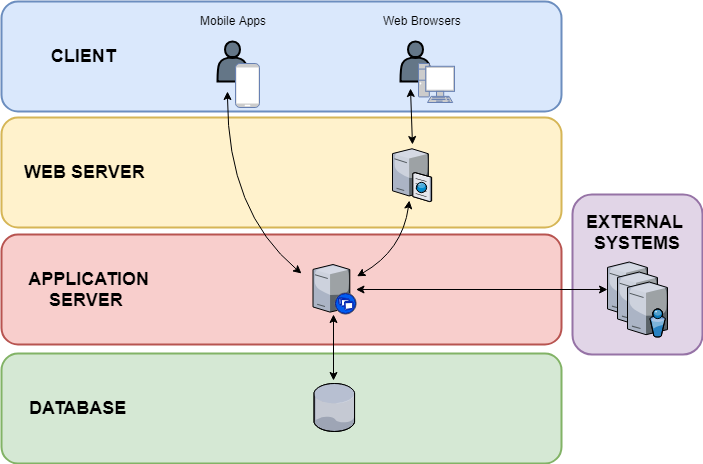
\includegraphics[width=\textwidth]{./img/LayeredStructure.png}
    \hspace{0.05\linewidth}
    \centering
    \caption{\textit{Layered Structure} of the system.}
		\label{img:layeredStructure}
    \end{center}
\end{figure}

The considered high-level components are:
\begin{itemize}
  \setlength{\itemindent}{-.4in}
  \item[] \textbf{Mobile Applications:} The \textit{Presentation Layer} dedicated to mobile devices; it communicates with the Application Server.
  \item[] \textbf{Web Browsers:} The \textit{Presentation Layer} dedicated to web browsers; it communicates directly with the Web Server.
  \item[] \textbf{Web Server:} This is the layer that provides web-pages for the web-based applications; it communicates with the Application Server and with the Web Browsers.
  \item[] \textbf{Application Server:} This is the layer in which is contained all the \textit{logic} for the application; it communicates with the Web Server and with the Database. Moreover it manages the communication with External Services.
  \item[] \textbf{Database:}  The \textit{Data Layer} of the system; it includes all structures and entities responsible for data storage and management. It communicates with the Application Server.
\end{itemize}
It has been taken the decision to separate the Application and Web Server in order to allow greater scalability. In the figure above it is also shown the interaction between the Application Server and External Systems.
A more detailed description of the intereactions between the described system components is shown in Figure \ref{img:highLevelComponents}.

\begin{figure}[H]
  \begin{center}
  	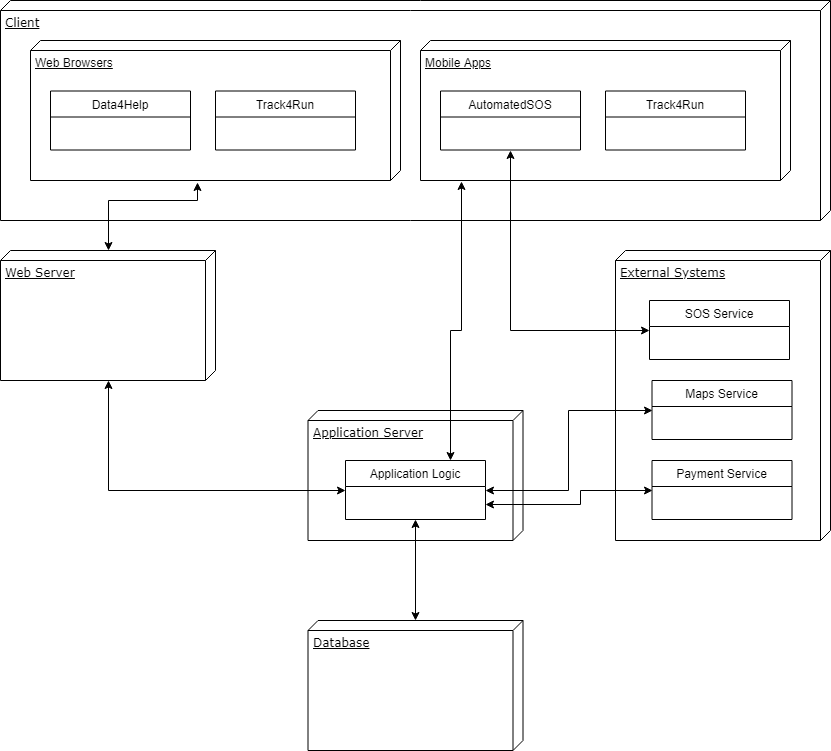
\includegraphics[width=\textwidth]{./img/HighLevelComponents.png}
    \hspace{0.05\linewidth}
    \centering
    \caption{\textit{High Level Components} of the system.}
		\label{img:highLevelComponents}
    \end{center}
\end{figure}

\section{Component View}
In this section the system will be described in term of its components. Functionalities of the components will be discussed and detailed will be shown the interfaces among components and among external services.

\subsection{Database}
The application database will be managed using a Relational DBMS.
It allows the reading of data, ensuring users the ability to log in and access the applications of interest and check the stored data.
It is also used for data manipulation (insertion, modification and deletion).
The use of a Relational DBMS guarantees the fundamental properties for a database of this type:
\begin{itemize}
  \item \textit{Atomicity}: no partial executions of operations.
  \item \textit{Consistency}: the database is always in a consistent state.
  \item \textit{Isolation}: each transaction is executed in an isolated and independent way.
  \item \textit{Durability / Persistence}: changes made are not lost.
\end{itemize}
The database will offer to the Application Server an interface that it can use to interact with the database.
The data stored in the database must be considered personal and confidential, therefore, procedures must be implemented to safeguard the stored information.\\
Particular attention must be paid to the reading permissions granted to users and to the encryption of passwords used to access the services offered.
Below is the designed E-R diagram.(Figure \ref{img:ER_Diagram})

\begin{figure}[H]
  \begin{center}
  	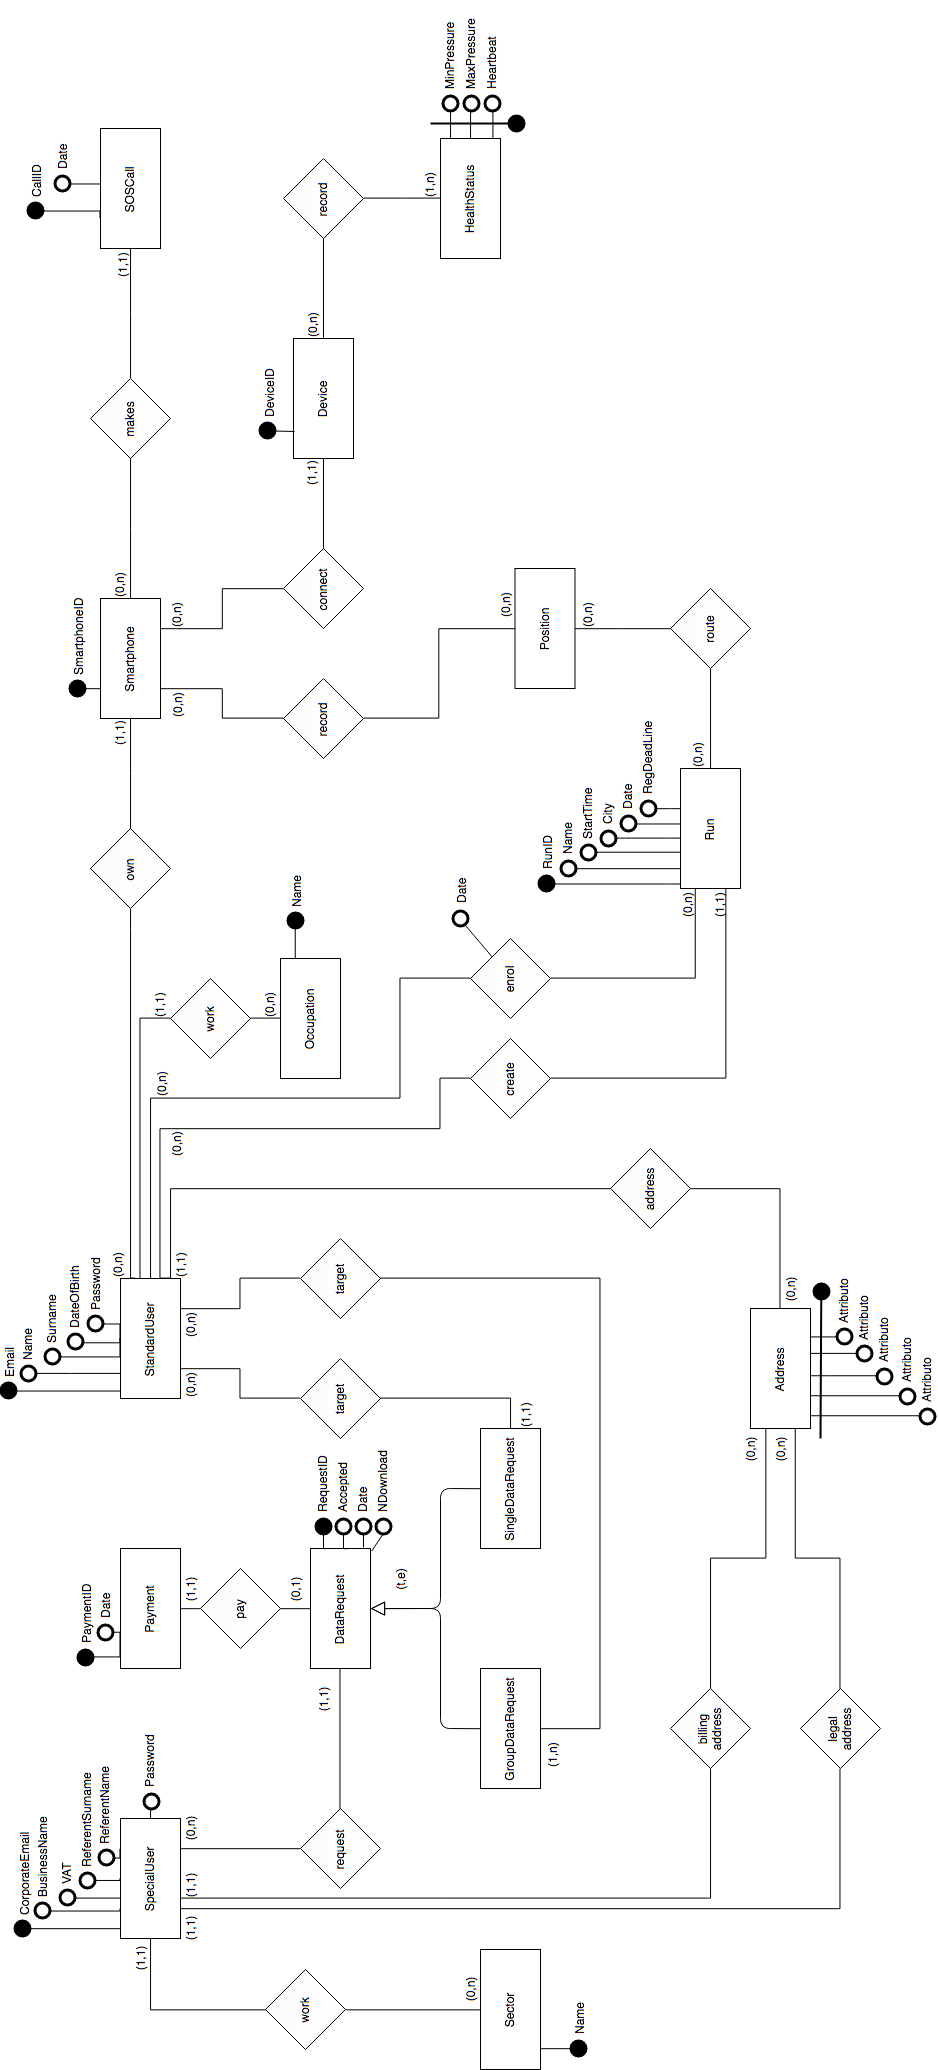
\includegraphics[height=0.68\paperheight]{./img/ER.png}
    \hspace{0.05\linewidth}
    \centering
    \caption{\textit{E-R} Diagram}
		\label{img:ER_Diagram}
    \end{center}
\end{figure}

\subsection{Application Server}
This is the crucial layer of the system to be. The main feature of the \textit{Application Server} is to describe rules and work-flows of all the functionalities provided by the application.\\
The \textit{Application Server} must have intefaces to communicate with the \textit{Web Server} and the \textit{Mobile Apps}, it has also to communicate through interfaces with all the \textit{External Services} (Maps Service, SOS Service and Payment Service).\\
Moreover, the \textit{Application Server} is the only entity of the system that is granted to communicate with the DBMS.
Following this brief introduction there are the logic modules and their descriptions, moreover all connections among components could be seen in the \textit{Global Component View} in Figure \ref{img:GlobalComponent}.

\paragraph{Data Collector Service}
This module offers the a service to the \textit{Standard User Manager} in order to maange user's data and store it into the \textit{Data4Help} database.

\paragraph{Group Request Manager}
This module manages the third party requests of \textit{Group Data Requirement}.

\paragraph{Mail Manager}
This module is a tool for other modules that allow the system to send e-mail, for instance in the registration and enrolment phase.

\paragraph{Maps Manager}
This module is an handler providing an interface to the external service of maps.

\paragraph{Payment Handler}
This module is an handler providing an interface to the external service of payment.

\paragraph{Persistence Unit}
This module is the unique interface to the database's DBMS.

\paragraph{Run Manager}
This module manages \textit{Runs} in all their functionalities, like creation, deletion and enrolment.\\
In order to manage guest users that visit a Run the system this module provides an access point to the \textit{Application Server} for the \textit{Web Server} and the \textit{Mobile Apps}.

\paragraph{Single Request Manager}
This module manages the third party requests of \textit{Single Data Requirement}.

\paragraph{Special User Manager}
This module provides all functionalities related to the \textit{Special User}.

\paragraph{Standard User Manager}
This module provides all functionalities related to the \textit{Standard User}.


\subsection{Mobile App}
The \textit{Mobile App} must communicate to the \textit{Application Server} through APIs that have to be defined in order to describe the interactions between the two layers and they must be indipendent from the implementation both side.\\
The App UI must be designed user friendly and it has to follow the guidelines provided by the Android and iOS producer.
The application must provide a software module that manages the GPS connection of the device and keeps track of locations data, it has also to manage the Health data from the devices connected to the phone.\\
The application must provide all collected data to the \textit{Application Server} in order to process them.

\subsection{AutomatedSOS App}
In this Section we want to specify in detail the modules that compose the \textit{AutomatedSOS} application in order to better explain the important activity of detection of possible \textit{Critical Situation}.\\
All connections among components could be seen in the \textit{AutomatedSOS Component View} in Figure \ref{img:AutomatedComponent}.

\paragraph{Application Server Handler}
This module is an handler providing an interface to the \textit{Application Server}.

\paragraph{Background Health Monitor}
This module checks status of health data that it receives. If an SOS call must be done it call \textit{SOS Handler}.

\paragraph{GUI}
This module is the \textit{Graphical} interface to the smartphone.

\paragraph{Health Status Service}
This module manage data detected and produce statistic for the \textit{User}.

\paragraph{SOS Handler}
This module is an handler providing an interface to the external service of SOS.

\subsection{Web Server}
The \textit{Web Server} must communicate to the \textit{Application Server} through HTTPS protocol.\\
The \textit{GUI} of the \textit{}{Web Server} must be designed user friendly and it has to follow the guidelines provided by W3C standard (using HTML5, CSS and JS).\\
The \textit{Control Unit} manages all actions played by a user and it must communicate to the \textit{Application Server} through APIs, that are already explained for the \textit{Mobile App}.

\begin{figure}[H]
  \begin{center}
  	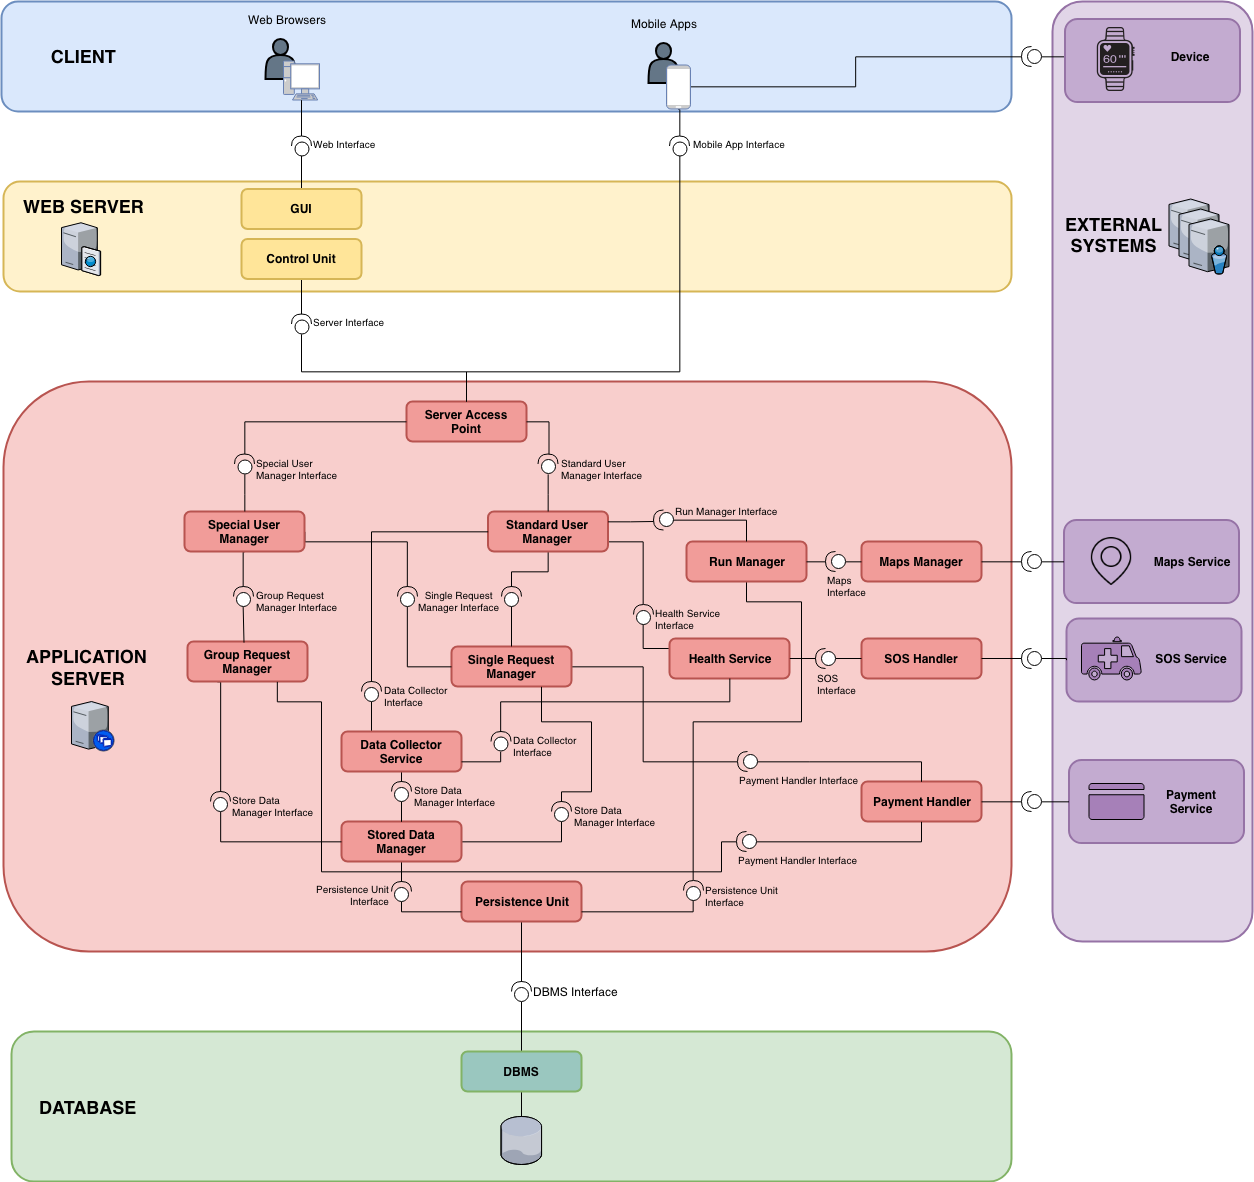
\includegraphics[width=\textwidth]{./img/GlobalComponent.png}
    \hspace{0.05\linewidth}
    \centering
    \caption{\textit{Global Component View}}
		\label{img:GlobalComponent}
    \end{center}
\end{figure}

\begin{figure}[H]
  \begin{center}
  	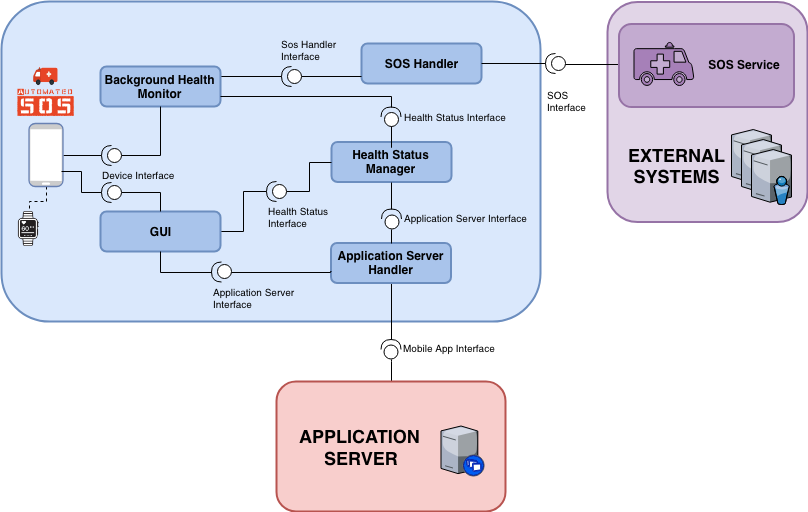
\includegraphics[width=\textwidth]{./img/Automated_Component.png}
    \hspace{0.05\linewidth}
    \centering
    \caption{\textit{AutomatedSOS Component View}}
		\label{img:AutomatedComponent}
    \end{center}
\end{figure}

\clearpage

\section{Deployment View}
Below is the deployment diagram of the system to be (Figure \ref{img:Deployment_Diagram}).

\begin{figure}[H]
  \begin{center}
  	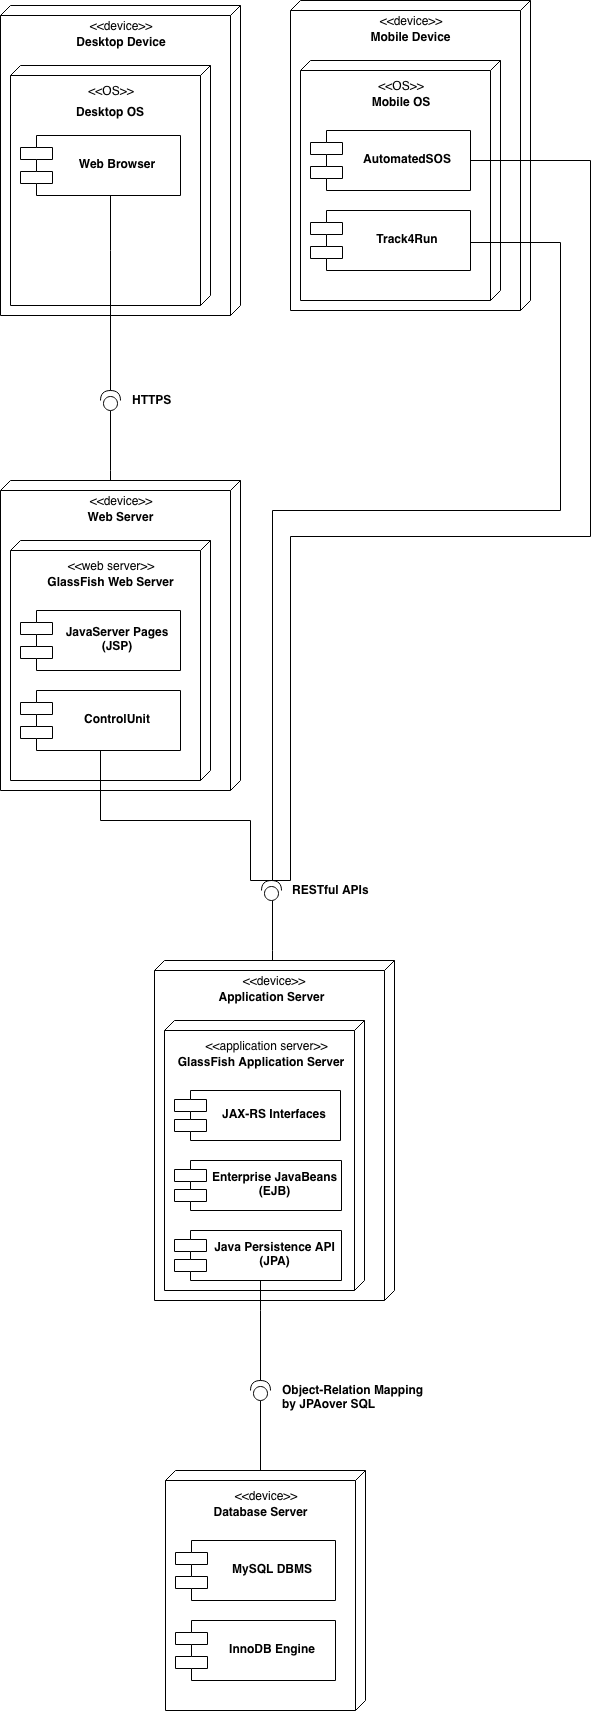
\includegraphics[height=0.59\paperheight]{./img/Deployment_Diagram.png}
    \hspace{0.05\linewidth}
    \centering
    \caption{Deployment Diagram of the system to be}
		\label{img:Deployment_Diagram}
    \end{center}
\end{figure}

\clearpage

\section{Runtime View}\label{runtimeViewSection}
In this Section we want to specify the behaviour of our system. Some relevant cases are selected and explained using Sequence Diagrams.

\begin{figure}[H]
  \begin{center}
  	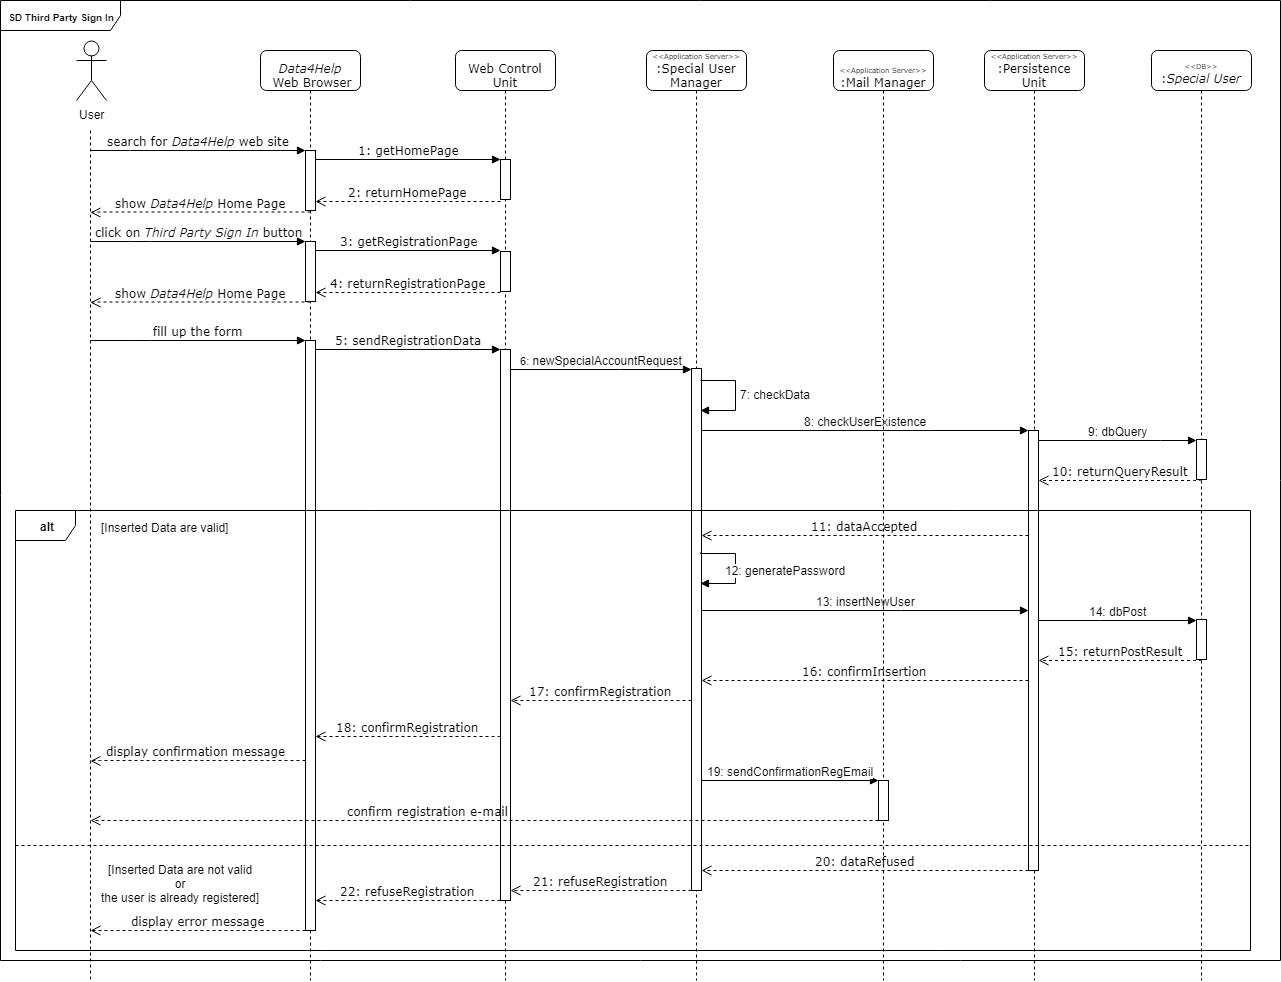
\includegraphics[width=\textwidth]{./img/sequence/webSignIn.png}
    \hspace{0.05\linewidth}
    \centering
    \caption{\textit{Third Party Sign In} sequence diagram: it is described the process through which a third party can register itself to \textit{Data4Help} services, obviously using \textit{Data4Help}'s web site, since it is the only available platform for third parties.}
		\label{img:webSignIn}
    \end{center}
\end{figure}

\begin{figure}[H]
  \begin{center}
  	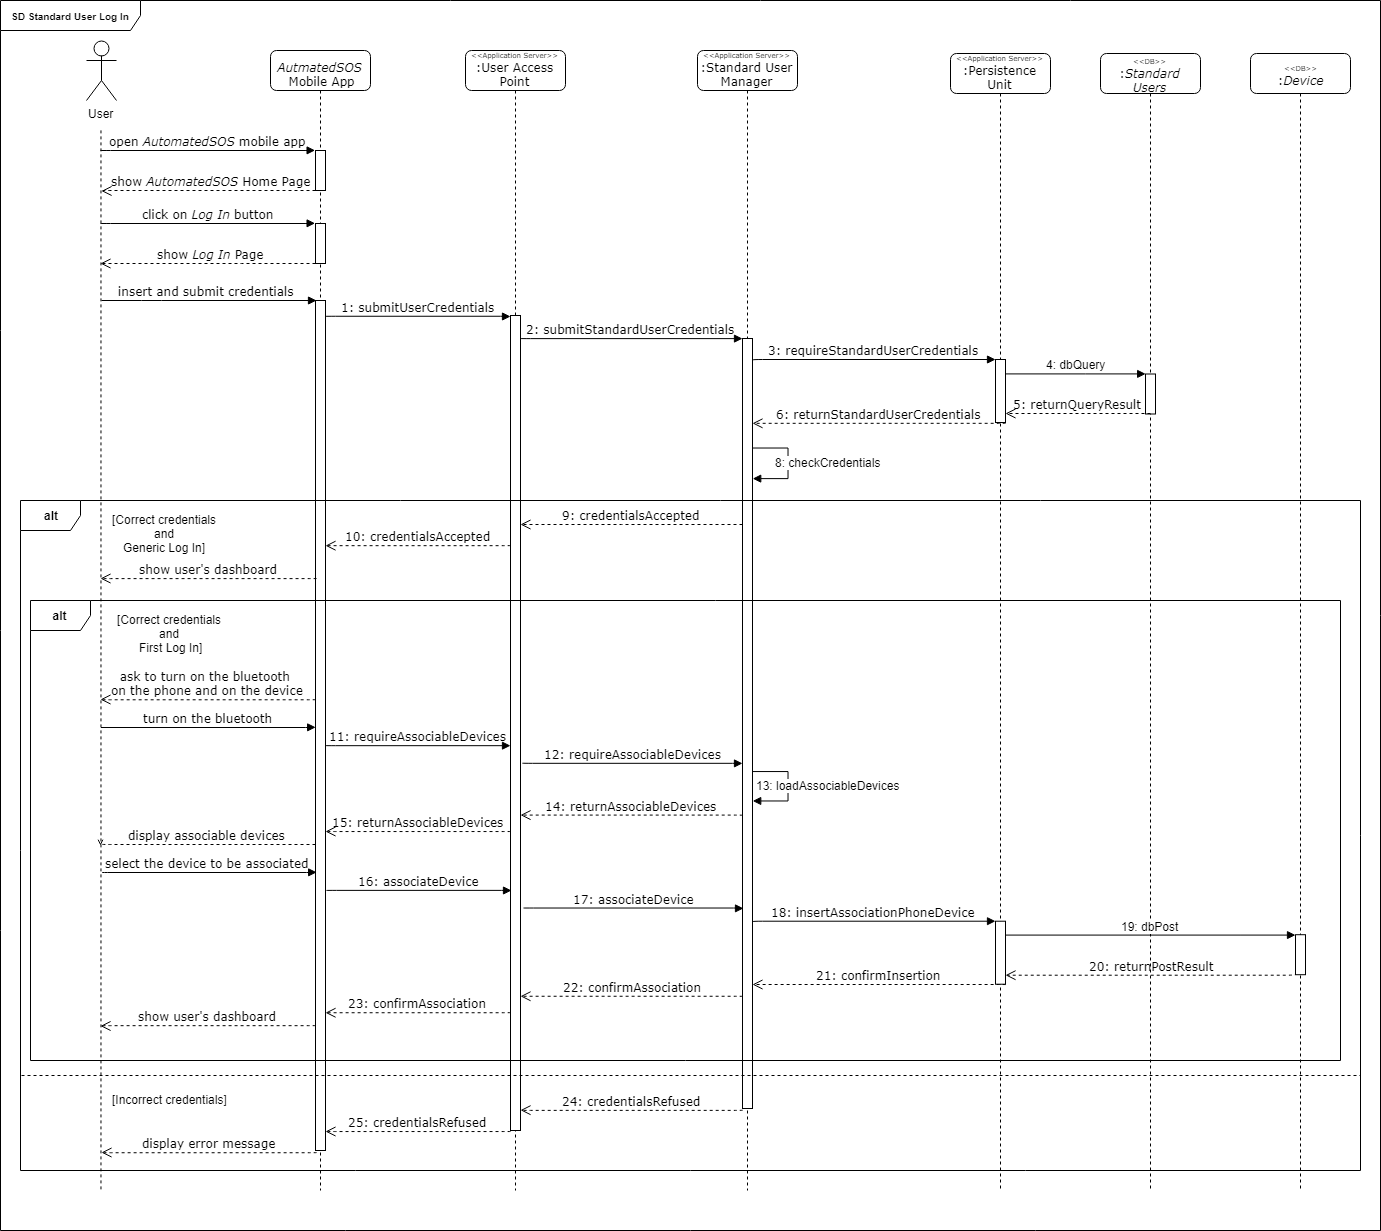
\includegraphics[width=\textwidth]{./img/sequence/appLogIn.png}
    \hspace{0.05\linewidth}
    \centering
    \caption{\textit{Standard User Log In} sequence diagram: it is described the process through which a standard user can access to \textit{AutomatedSOS} or \textit{Track4Run} applications.}
		\label{img:appLogIn}
    \end{center}
\end{figure}

\begin{figure}[H]
  \begin{center}
  	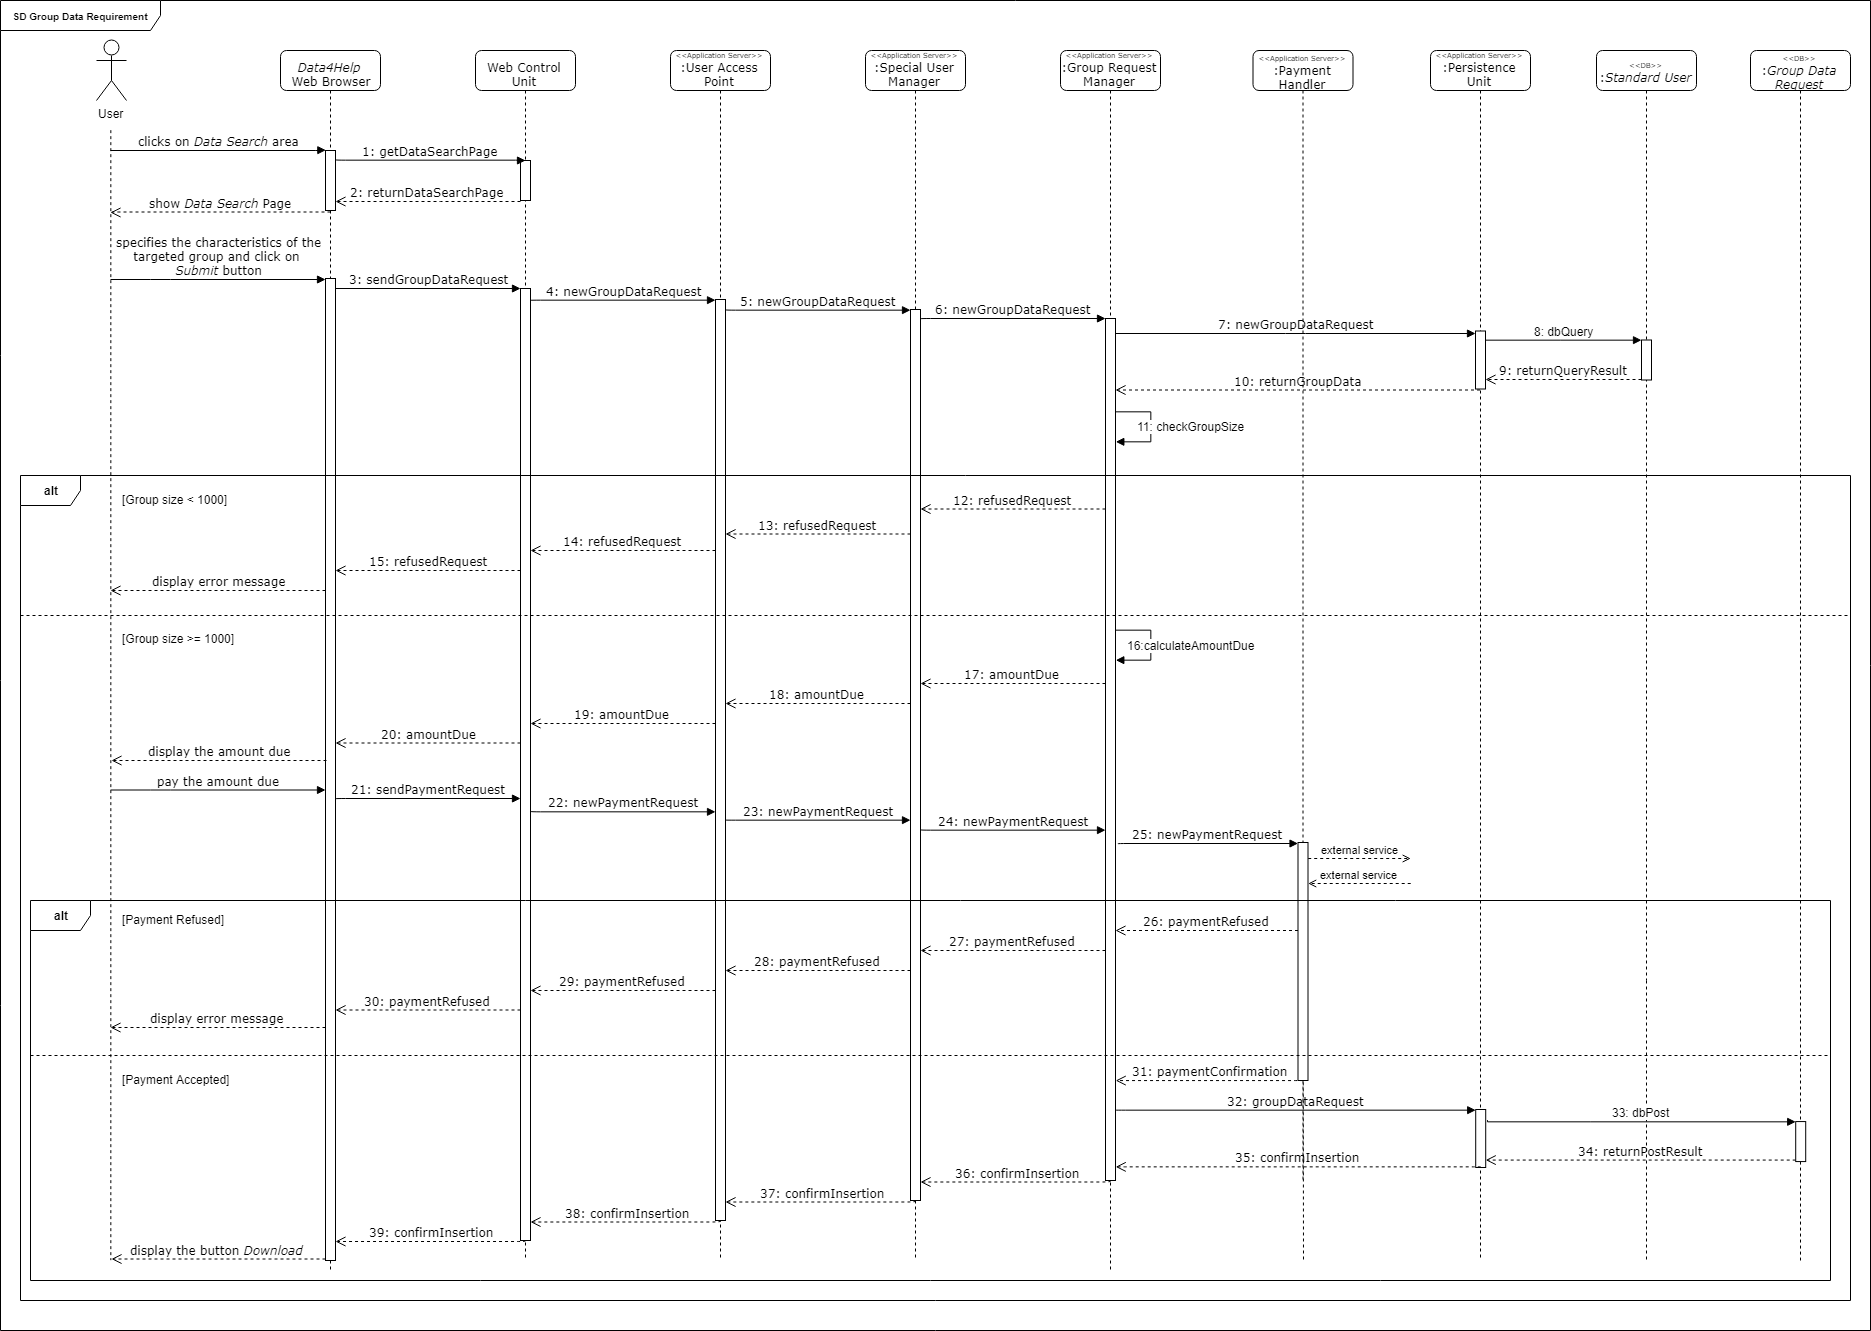
\includegraphics[width=\textwidth]{./img/sequence/groupDataRequest.png}
    \hspace{0.05\linewidth}
    \centering
    \caption{\textit{Group Data Request} sequence diagram: it is described the process through which a third party can require data of a group of people and then pay them.}
		\label{img:groupDataRequest}
    \end{center}
\end{figure}

\begin{figure}[H]
  \begin{center}
  	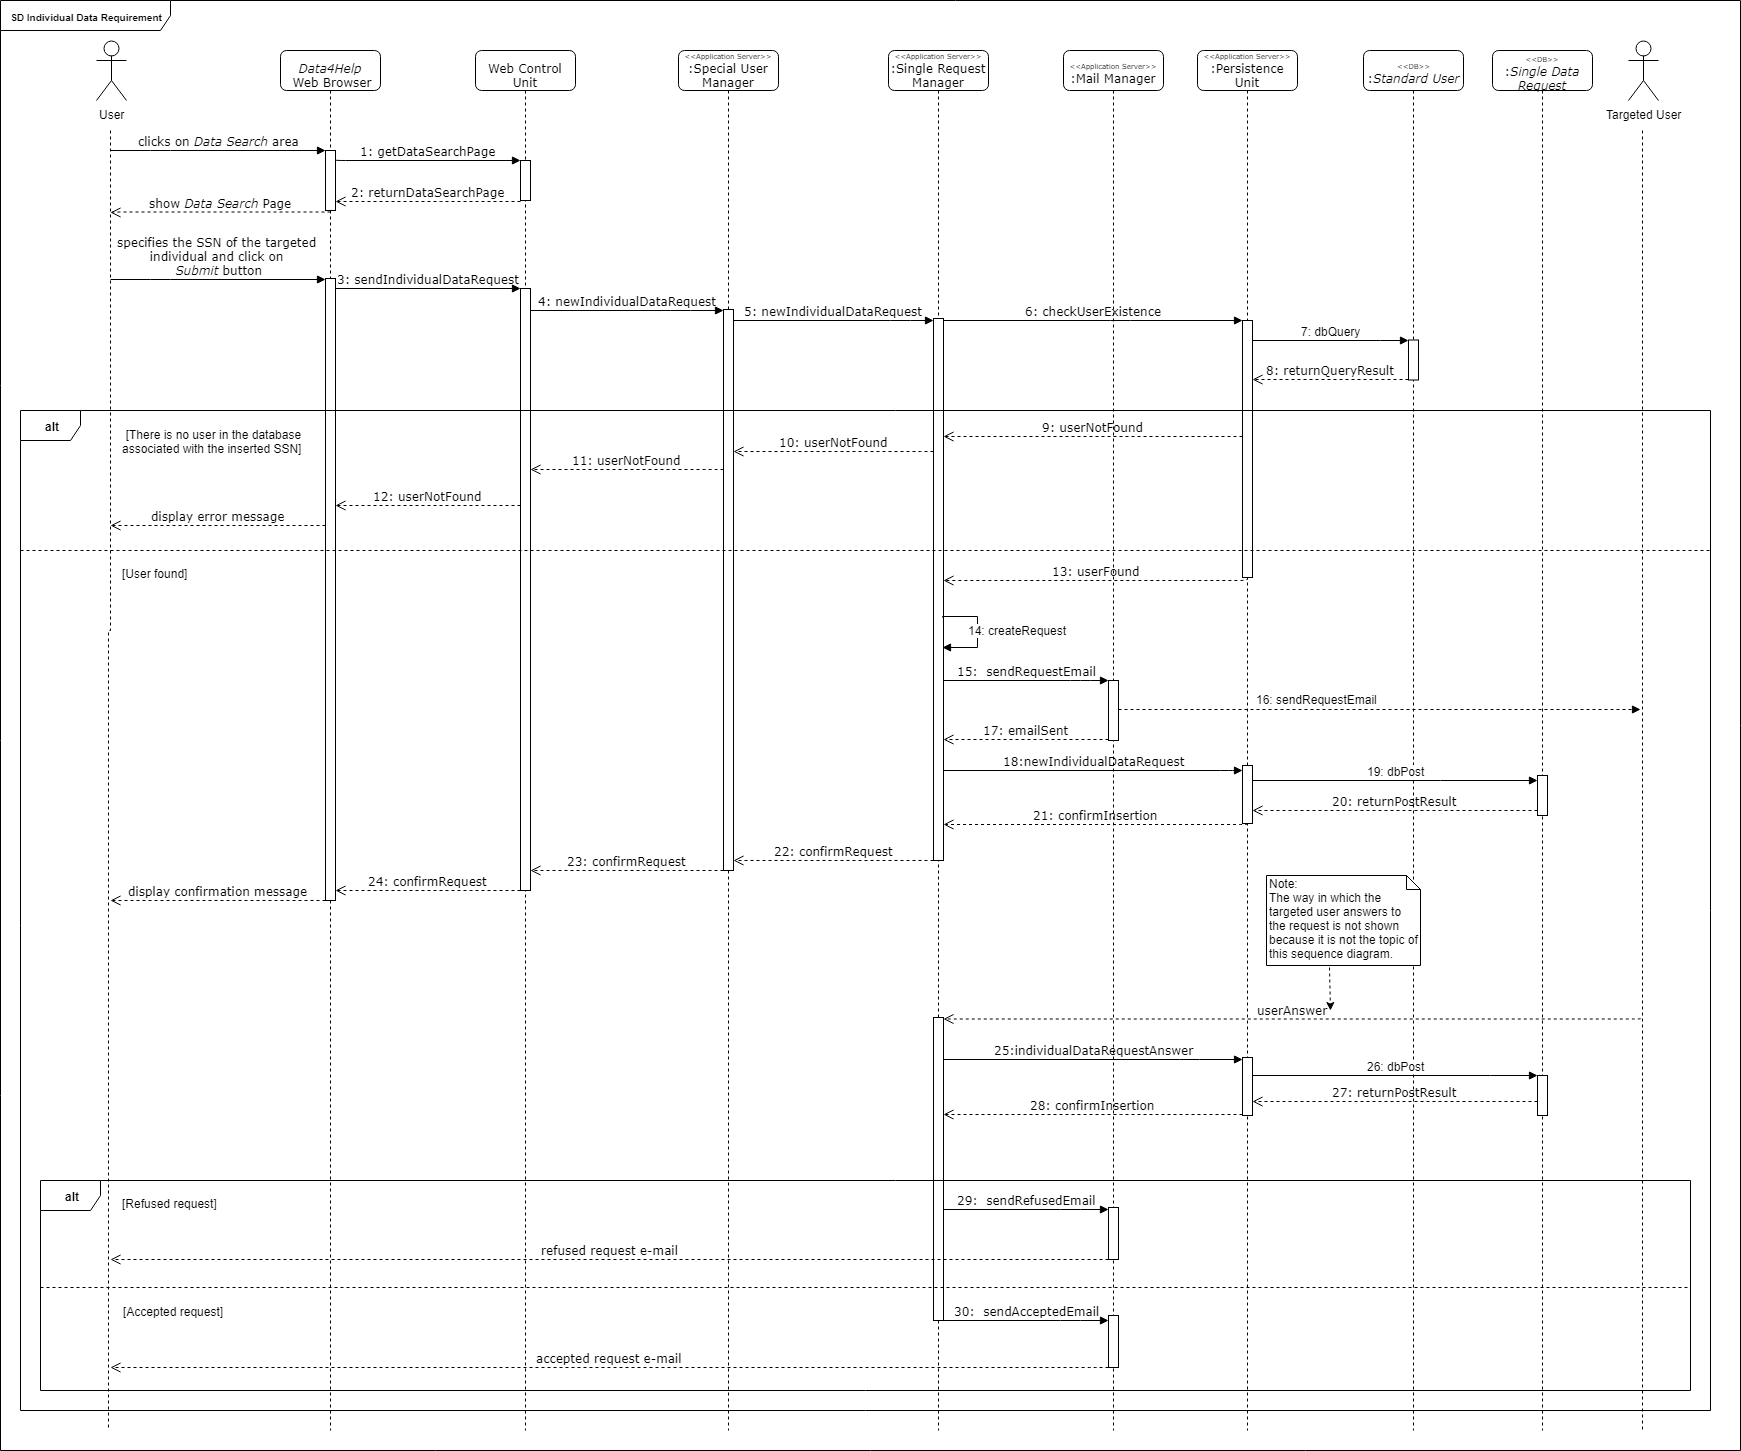
\includegraphics[width=\textwidth]{./img/sequence/individualDataRequest.png}
    \hspace{0.05\linewidth}
    \centering
    \caption{\textit{Individual Data Request} sequence diagram: it is described the process through which a third party can require data of an individual user and wait for a response. It is not described the way in which the targeted user answers to the request because it is not the topic of this sequence diagram. It is not even described the way in which the third party pays and eventually downloads the data because it is not considerable and it has just been explained in the \textit{Group Data Requst} sequence diagram.}
		\label{img:individualDataRequest}
    \end{center}
\end{figure}

\begin{figure}[H]
  \begin{center}
  	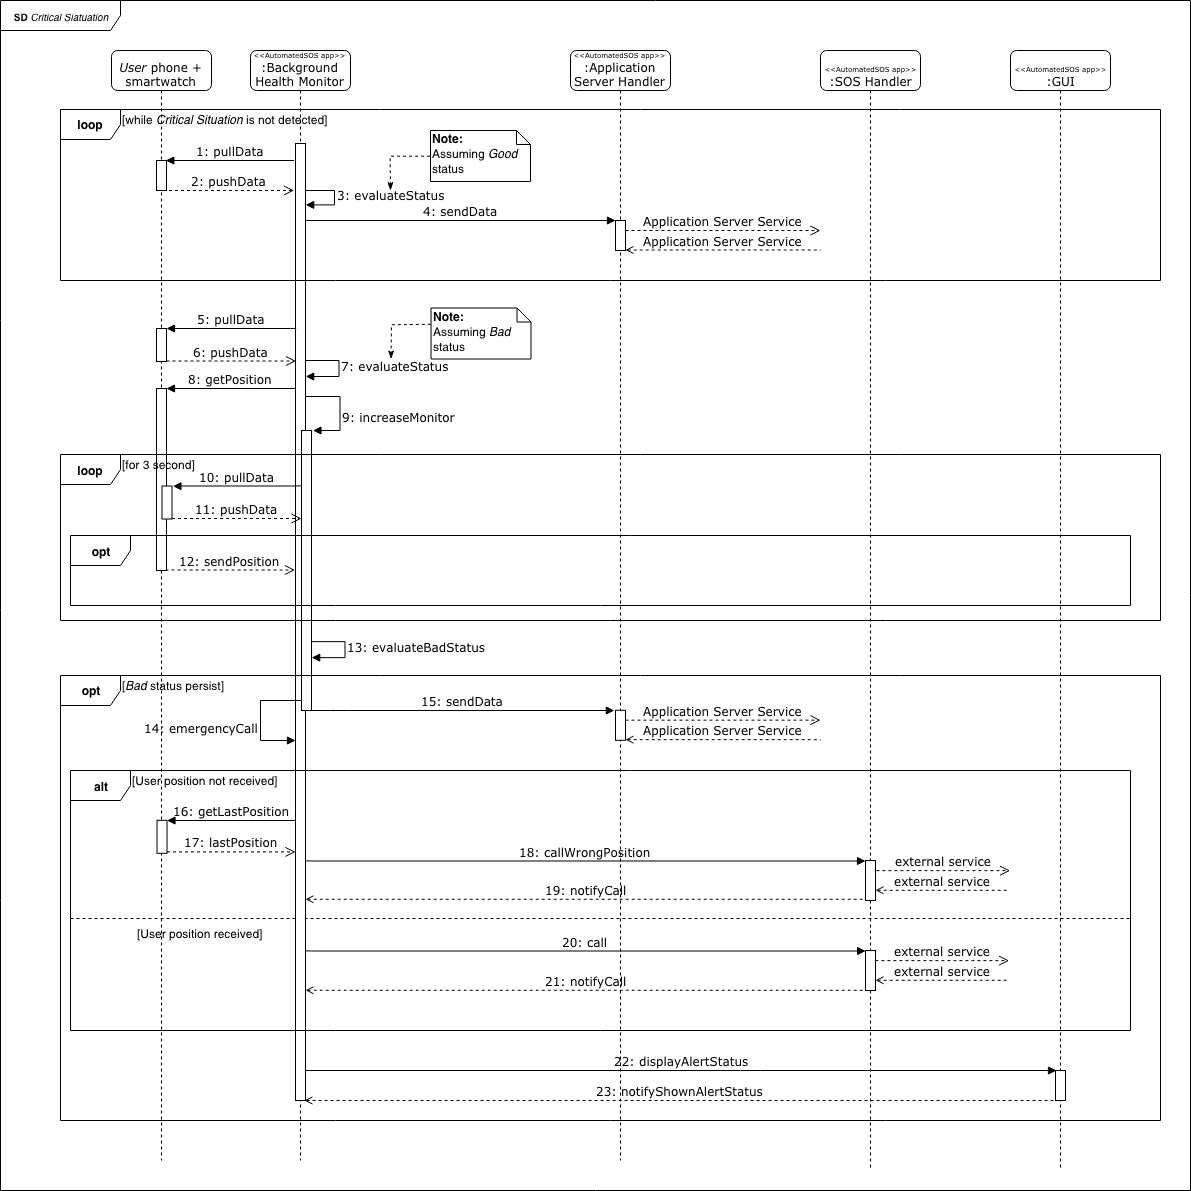
\includegraphics[width=\textwidth]{./img/sequence/criticalSituation.png}
    \hspace{0.05\linewidth}
    \centering
    \caption{\textit{Critical Situation} sequence diagram: it is described the process through which a critical situation is detected by \textit{AutomatedSOS} application + device. It is not described the way in which \textit{AutomatedSOS} application stored the acquired data because it is not considerable for this topic.}
		\label{img:criticalSituation}
    \end{center}
\end{figure}

\begin{figure}[H]
  \begin{center}
  	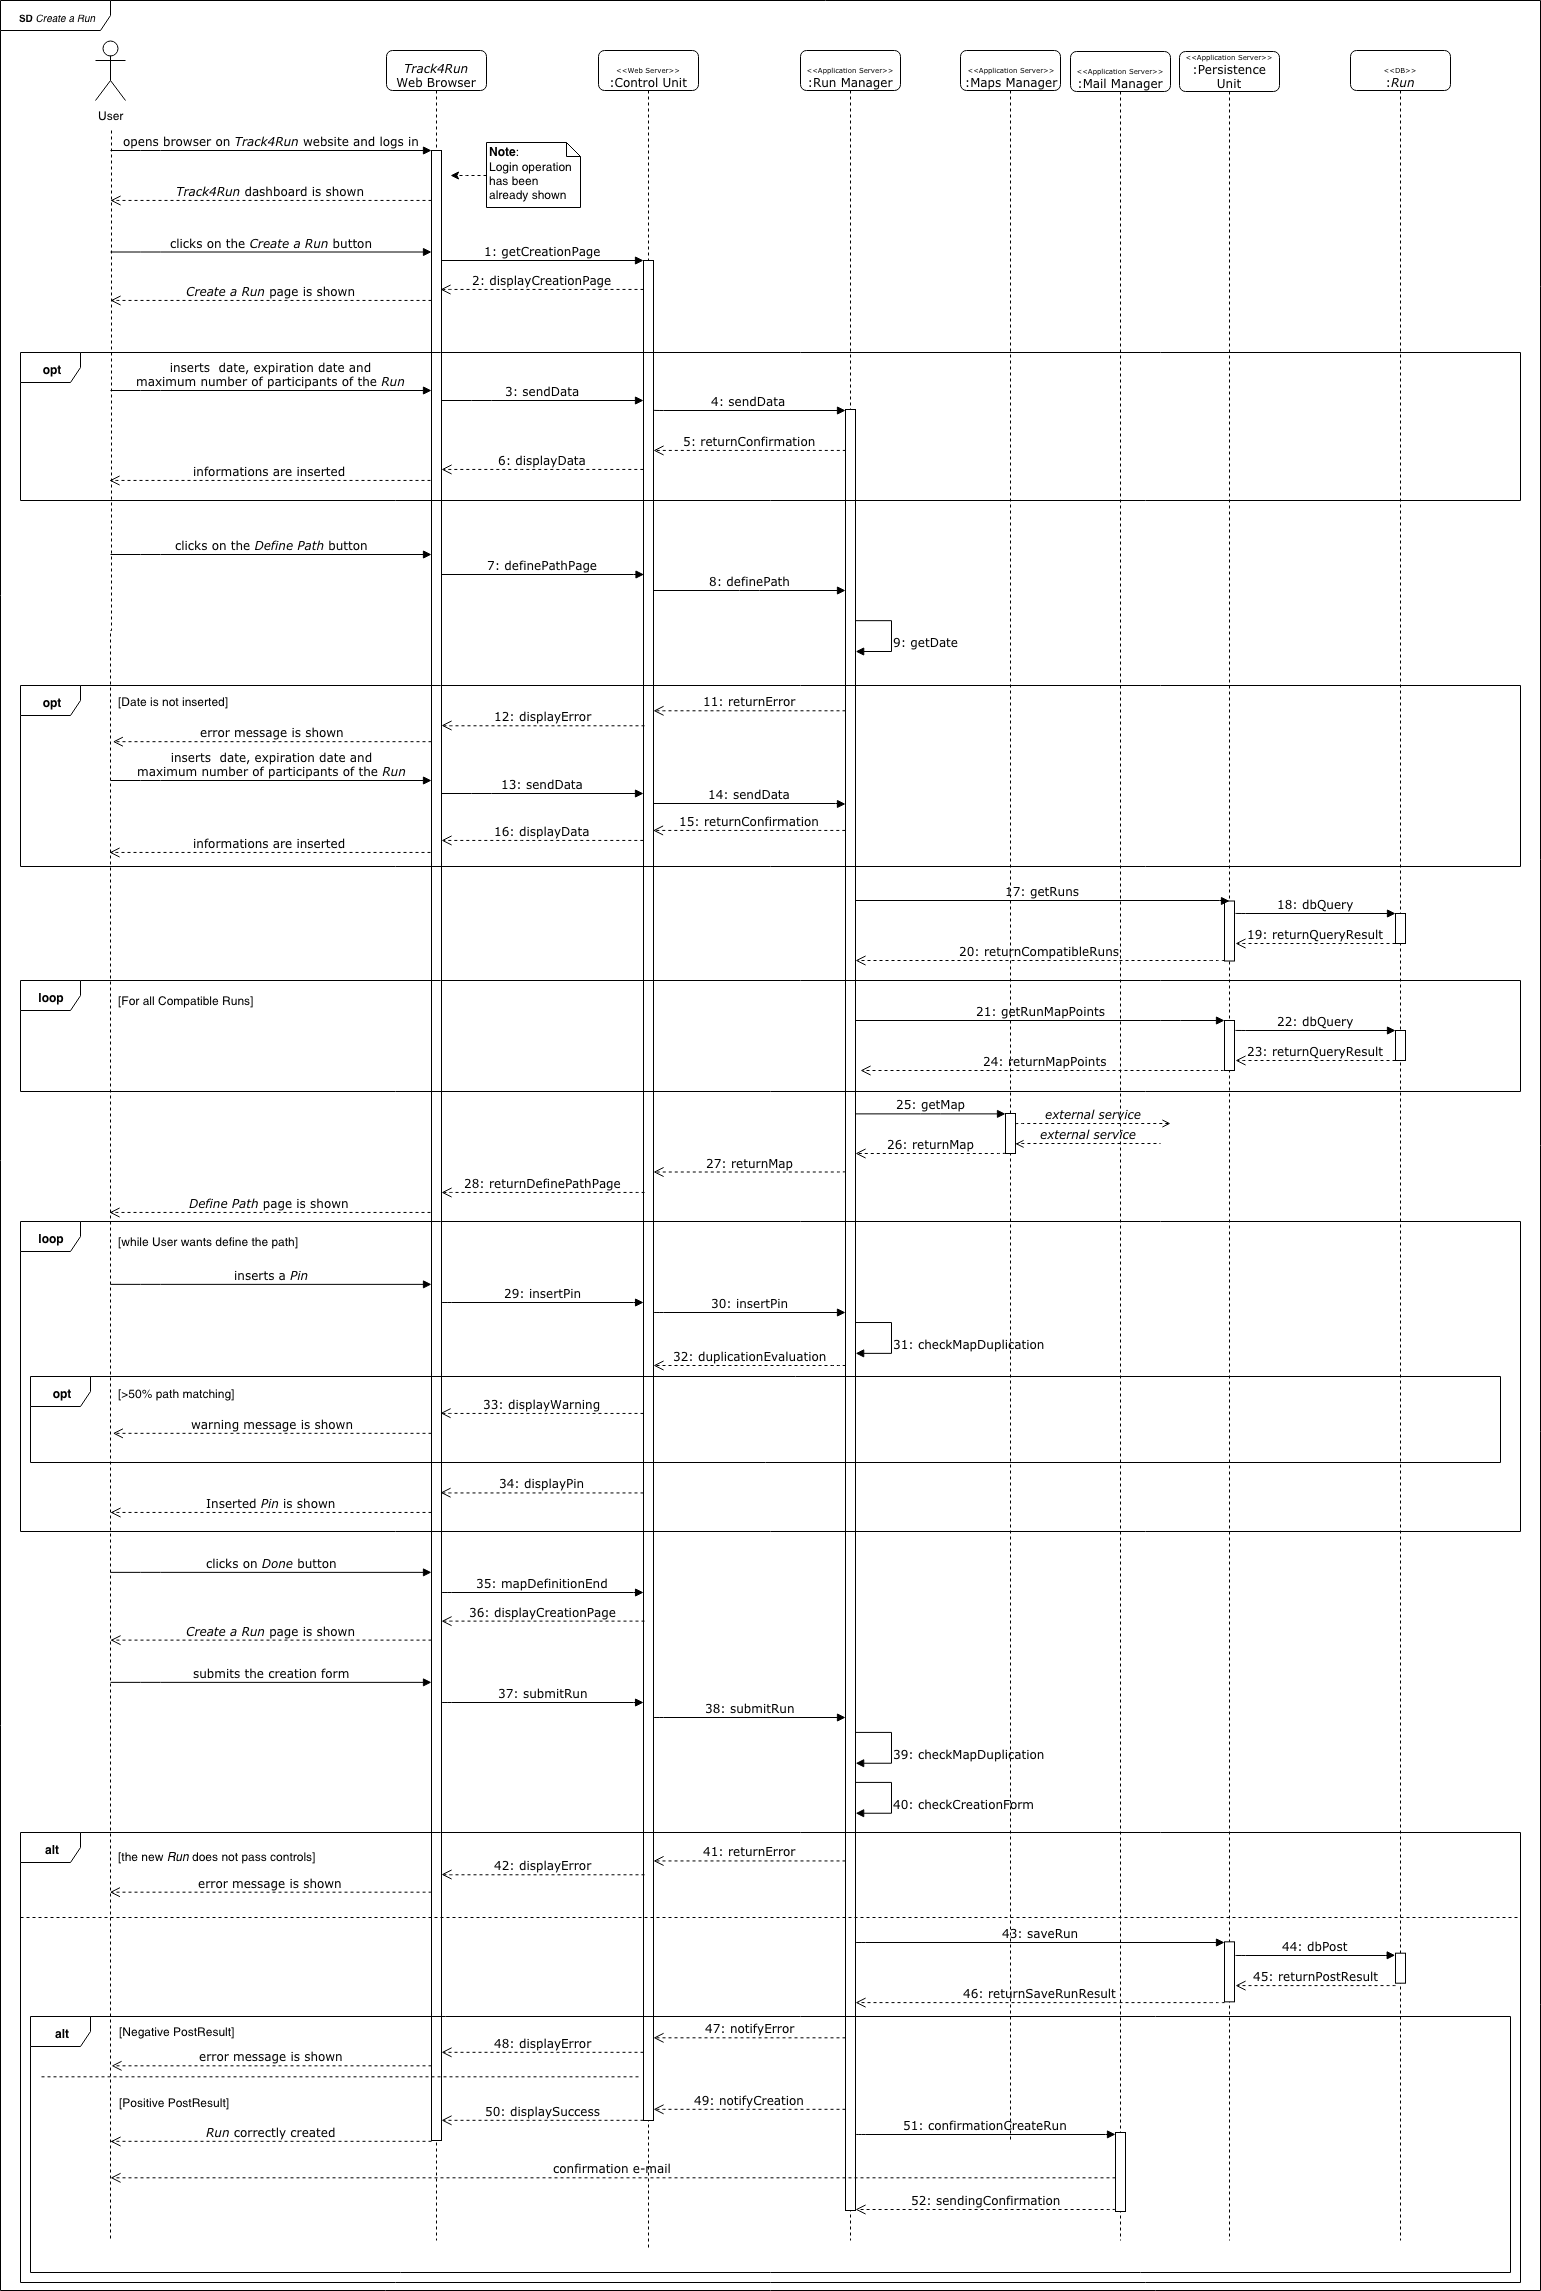
\includegraphics[height=.6\paperheight]{./img/sequence/createRun.png}
    \hspace{0.05\linewidth}
    \centering
    \caption{\textit{Create a Run} sequence diagram: it is described the process through which a standard user can create a new run.}
		\label{img:createRun}
    \end{center}
\end{figure}

\begin{figure}[H]
  \begin{center}
  	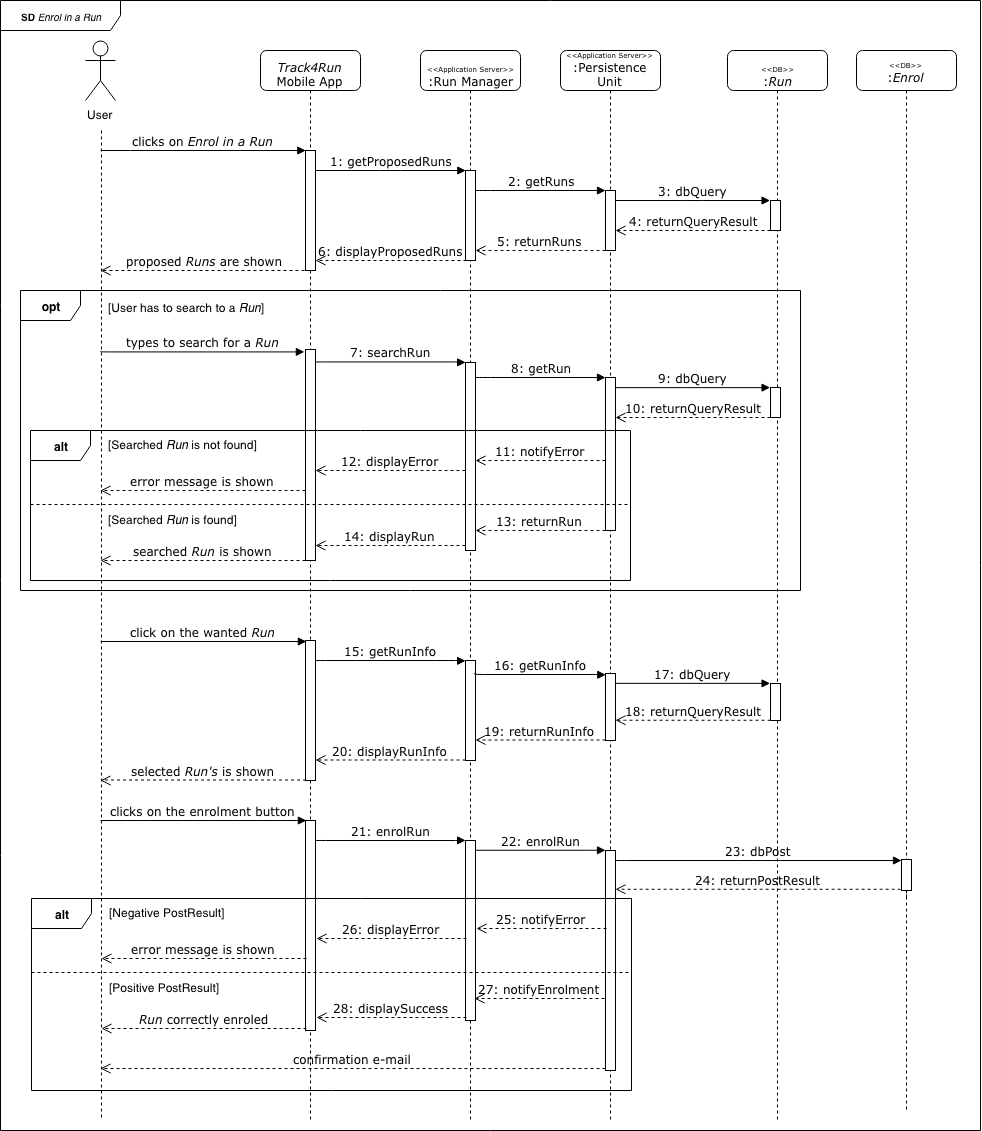
\includegraphics[width=\textwidth]{./img/sequence/enrolRun.png}
    \hspace{0.05\linewidth}
    \centering
    \caption{\textit{Enrol in a Run} sequence diagram: it is described the process through which a standard user can enrol himself/herself in a run. }
		\label{img:enrolRun}
    \end{center}
\end{figure}

\begin{figure}[H]
  \begin{center}
  	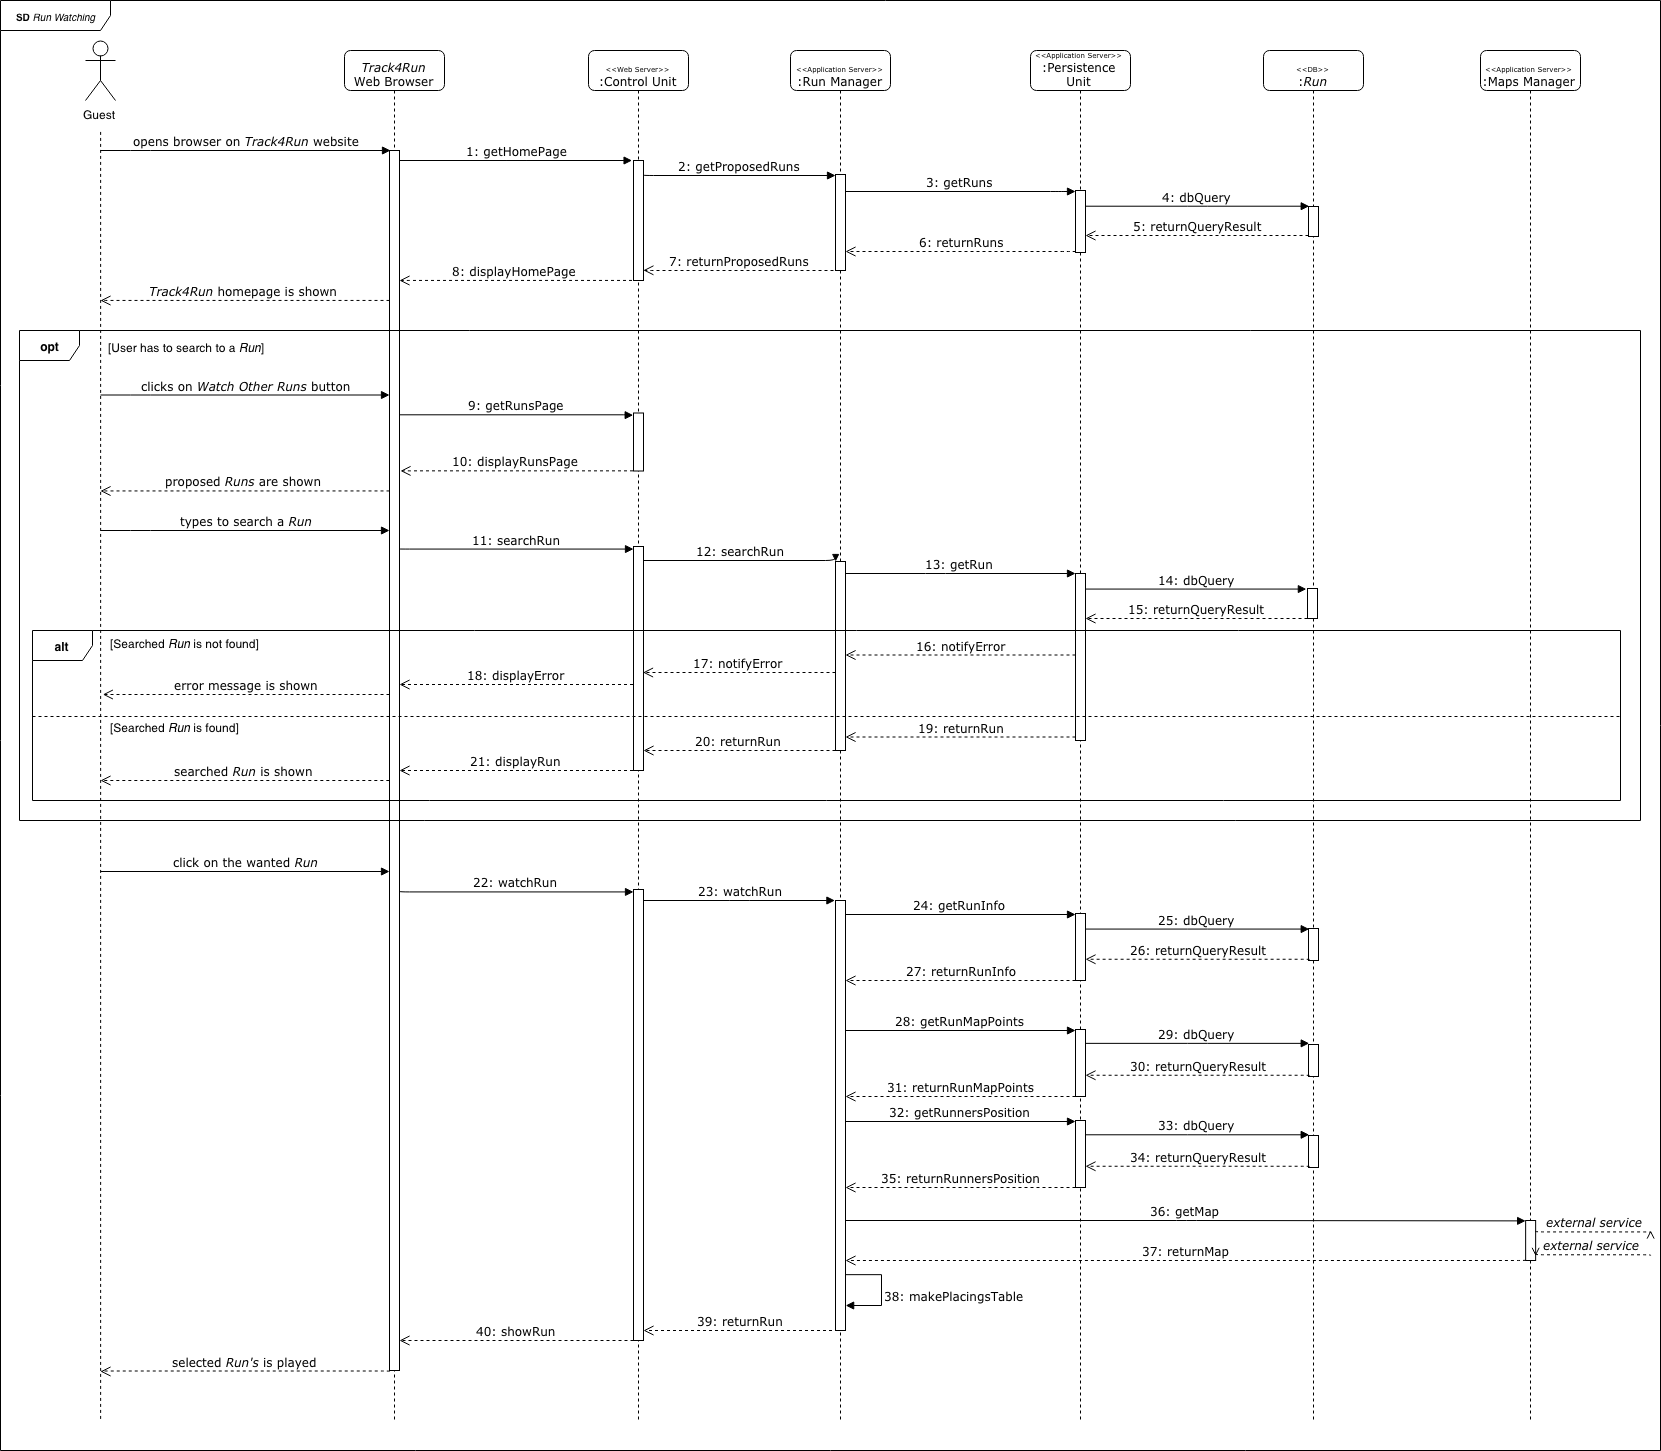
\includegraphics[width=\textwidth]{./img/sequence/watchRun.png}
    \hspace{0.05\linewidth}
    \centering
    \caption{\textit{Run Watching} sequence diagram: it is described the process through which a not registered user can watch a run. Notice that he/she can access directly to part of the \textit{Run Manager} services without any log in.}
		\label{img:watchRun}
    \end{center}
\end{figure}


\clearpage

\section{Component Interfaces}
This section contains some detailed informations about interfaces between components of the system.\\
A detailed description focuses the attention over the actions of a procedure of a certain component called by other components.\\
Huge part of these actions could be seen played in the \textit{Sequence Diagrams} (Section \ref{runtimeViewSection}).

\subsection{Application Server}

\subsubsection{Standard User Manager}
Following procedures are called by other components:
\begin{itemize}
  \item \textbf{associateDevice}\quad This procedure is used to associate a selected device with the smartphone in use.
  \item \textbf{changeDevice}\quad This procedure is called to start the process of changing the associated device.
  \item \textbf{changePassowrd}\quad This procedure is called to change the password of the user's account.
  \item \textbf{deleteProfile}\quad This procedure is called to delete the user's profile.
  \item \textbf{modifyPersonalInformations}\quad This procedure is called to modify personal informations (among the modifiable ones:  city of residence, address and occupation.)
  \item \textbf{newStandardAccountRequest}\quad This procedure is called to start a standard user registration process that can be then accepted or refused.
  \item \textbf{requireAssociableDevices}\quad This procedure is used to induce the system to load the list of associable devices.
  \item \textbf{submitStandardUserCredentials}\quad This procedure is called to let (or not) a standard user log in into one of \textit{Track Me} services.
\end{itemize}

\myparagraph{}
Following procedures are called internally to the component:
\begin{itemize}
  \item \textbf{checkCredentials}\quad This procedure is called to check whether the credentials inserted by the user during the login match with the ones saved in the system's database.
  \item \textbf{checkData}\quad This procedure is called to check if the user has inserted correctly all the required data.
  \item \textbf{generatePassword}\quad This procedure is called to generate a random password to be assigned to the newly created standard user.
  \item \textbf{loadAssociableDevices}\quad This procedure is called to load the list of associable devices.
\end{itemize}

\subsubsection{Special User Manager}
Following procedures are called by other components:
\begin{itemize}
  \item \textbf{changePassowrd}\quad This procedure is called to change the password of the special user's account.
  \item \textbf{deleteProfile}\quad This procedure is called to delete the user's profile.
  \item \textbf{modifyPersonalInformations}\quad This procedure is called to modify personal informations (among the modifiable ones:  legal address, billing address, corporate e-mail address, sector and all the data regarding the legal representative)
  \item \textbf{newGroupDataRequest}\quad This procedure is called to start the process of requiring data of a group of people and to send the useful data to the specialized component (\textit{Group Request Manager}).
  \item \textbf{newIndividualDataRequest}\quad This procedure is called to start the process of requiring to an individual user the sharing of his/her data and to send the useful data to the specialized component (\textit{Single Request Manager}).
  \item \textbf{newPaymentRequest}\quad This procedure is called to start the process of paying some required data calling the corresponding procedure on the more specialized component (\textit{Group Request Manager}).
  \item \textbf{newSpecialAccountRequest}\quad This procedure is called to start a special user registration process that can be then accepted or refused.
  \item \textbf{submitSpecialUserCredentials}\quad This procedure is called to let (or not) a special user log in into one of \textit{Track Me} services.
\end{itemize}

\myparagraph{}
Following procedures are called internally to the component:
\begin{itemize}
  \item \textbf{checkCredentials}\quad This procedure is called to check whether the credentials inserted by the special user during the login match with the ones saved in the system's database.
  \item \textbf{checkData}\quad This procedure is called to check if the special user has inserted correctly all the required data.
  \item \textbf{generatePassword}\quad This procedure is called to generate a random password to be assigned to the newly created special user.
\end{itemize}

\subsubsection{Group Request Manager}
Following procedures are called by other components:
\begin{itemize}
  \item \textbf{newGroupDataRequest}\quad This procedure is called to start the process of requiring data of a group of pepole.
  \item \textbf{newPaymentRequest}\quad This procedure is called to start the process of paying some required data calling the corresponding procedure on the dedicated component (\textit{Payment Handler}).
\end{itemize}

\myparagraph{}
Following procedures are called internally to the component:
\begin{itemize}
  \item \textbf{calculateAmountDue}\quad This procedure is called to calculate the amount due to download some required available data.
  \item \textbf{checkGroupSize}\quad This procedure is called to check whether the size of the required group of people is over 10000 or not.
\end{itemize}

\subsubsection{Single Request Manager}
Following procedures are called by other components:
\begin{itemize}
  \item \textbf{newIndividualDataRequest}\quad This procedure is called to start the process of requiring to an individual user the sharing of his/her data.
  \item \textbf{newPaymentRequest}\quad This procedure is called to start the process of paying some required data calling the corresponding procedure on the dedicated component (\textit{Payment Handler}).
\end{itemize}

\myparagraph{}
Following procedures are called internally to the component:
\begin{itemize}
  \item \textbf{calculateAmountDue}\quad This procedure is called to calculate the amount due to download some required available data.
  \item \textbf{createRequest}\quad This procedure is called to generate a sharing data request that has to be sent to an individual user.
\end{itemize}

\subsubsection{Mail Manager}
Following procedure is called by other components:
\begin{itemize}
  \item \textbf{confirmationEmail}\quad This procedure sends a confirmation e-mail to the user.
  \item \textbf{sendAcceptedEmail}\quad This procedure is called to inform a third party that an individual user, of which it has required the data, has accepted its request and so data will be immediatly available after completing the payment.
  \item \textbf{sendRefusedEmail}\quad This procedure is called to inform a third party that an individual user, of which it has required the data , has refused its request.
  \item \textbf{sendRequestEmail}\quad This procedure is called to send a sharing data request to an individual user.
\end{itemize}

\subsubsection{Maps Manager}
Following procedure is called by other components:
\begin{itemize}
  \item \textbf{getMap}\quad This procedure retrives a map from the external service.
\end{itemize}

\subsubsection{Run Manger}
Following procedures are called by other components:
\begin{itemize}
  \item \textbf{checkCreationForm}\quad This procedure checks all the fields of a creation for \textit{Create a Run} form.
  \item \textbf{definePath} \quad This procedure is called to open the path definition interface and to prepare the system to manage avoiding of maps duplications.
  \item \textbf{deleteEnrolement} \quad This procedure allow a user to delete an enrolment in a \textit{Run}.
  \item \textbf{deleteRun} \quad This procedure allow a user to delete a \textit{Run}.
  \item \textbf{enrolRun} \quad This procedure allow a user to enrol in a \textit{Run}.
  \item \textbf{getProposedRuns} \quad This procedure is called to retrive \textit{Runs} to propose to the users.
  \item \textbf{getRunInfo} \quad This procedure is called to retrive information of a particular \textit{Run}.
  \item \textbf{insertPin} \quad This procedure is called to insert a \textit{Pin} on a map during hte definition of a path.
  \item \textbf{makePlacingsTable} \quad This procedure is called to create the \textit{Placings Table} of a given \textit{Run} knowing path and runners' position.
  \item \textbf{searchRun} \quad This produce is called to search a given \textit{Run}.
  \item \textbf{sendData} \quad This procedure is used to submit data informations of a \textit{Run} and these data are used to compute functional requirement expecially for the \textit{Create a Run} use case (for instance avoiding 50\% of map duplication).
  \item \textbf{submitRun} \quad This produce is called when a \textit{User} has defined a \textit{Run} and wants to publish it.
  \item \textbf{watchRun} \quad This procedure is called to watch a given \textit{Run}.
\end{itemize}

\myparagraph{}
Following procedures are called internally to the component.
\begin{itemize}
  \item \textbf{checkMapDuplication} \quad This procedure is called to check the duplication of a given path with the compatible ones.
  \item \textbf{getDate} \quad This procedure is used to get the inserted \textit{Date} during the \textit{Create a Run} phase.
\end{itemize}

\subsubsection{Persistence Unit}
Following procedures are called by other components:
\begin{itemize}
  \item \textbf{checkExistingUser}\quad This procedure queries the credentials of a specific user to check whether they are already present in the database or not.
  \item \textbf{deleteEnrolement} \quad This procedure deletes an enrolment of a user on the DB through the DBMS.
  \item \textbf{deleteRun} \quad This procedure deletes a \textit{Run} on the DB through the DBMS.
  \item \textbf{enrolRun}\quad This procedure posts an enrolment of a user on the DB through the DBMS.
  \item \textbf{getRun}\quad This procedure queries required \textit{Run} on the DB through the DBMS.
  \item \textbf{getRunInfo}\quad This procedure queries required \textit{Run}'s information on the DB through the DBMS.
  \item \textbf{getRunMapPoints}\quad This procedure queries required \textit{Run path} on the DB through the DBMS.
  \item \textbf{getRunnersPosition}\quad This procedure queries \textit{Runners} position of a certain \textit{Run} on the DB through the DBMS.
  \item \textbf{getRuns}\quad This procedure queries required \textit{Runs} on the DB through the DBMS.
  \item \textbf{groupData}\quad This procedure queries the data of a specified group of people on the DB through the DBMS.
  \item \textbf{individualDataRequestAnswer}\quad This procedure posts the answer recieved by an individual user for an individual data request on the DB through the DBMS.
  \item \textbf{insertAssociationPhoneDevice}\quad This procedure posts a new association phone-device on the DB through the DBMS.
  \item \textbf{insertNewUser}\quad This procedure posts a new user on the DB through the DBMS.
  \item \textbf{newGroupDataRequest}\quad This procedure posts a new group data request on the DB through the DBMS.
  \item \textbf{newIndividualDataRequest}\quad This procedure posts a new individual data request on the DB through the DBMS.
  \item \textbf{requireSpecialUserCredentials}\quad This procedure queries the credentials of a special user (its email-password) to check if they correspond with the ones inserted during the login.
  \item \textbf{requireStandardUserCredentials}\quad This procedure queries the credentials of a standard user (his/her email-password) to check if they correspond with the ones inserted during the login.
  \item \textbf{saveRun}\quad This procedure posts a new \textit{Run} on the DB through the DBMS.
\end{itemize}

\subsubsection{Payment Handler}
Following procedures is called by other components:
\begin{itemize}
  \item \textbf{newPaymentRequest}\quad This procedure is called to pay some required data, it calls the dedicated external service.
\end{itemize}

\subsection{AutomatedSOS}
\subsubsection{Application Server Handler}
Following procedures are called by other components:
\begin{itemize}
  \item \textbf{getData}\quad This procedure is called to get data information of the user from the DB via \textit{Application Server}.
  \item \textbf{login}\quad This procedure is called to log in \textit{AutomatedSOS}.
  \item \textbf{sendData}\quad This procedure is called to send data information of the user to the \textit{Application Server} and store them into the DB.
\end{itemize}

\subsubsection{Background Health Monitor}
Following procedures are called by other components:
\begin{itemize}
  \item \textbf{lastPosition}\quad This procedure is called to send the last \textit{User}'s position to \textit{AutomatedSOS}.
  \item \textbf{pushData}\quad This procedure is called to send data that \textit{AutomatedSOS} has to evaluate.
  \item \textbf{sendPosition}\quad This procedure is called to send user's position to \textit{AutomatedSOS}.
\end{itemize}

\myparagraph{}
Following procedures are called internally to the component.
\begin{itemize}
  \item \textbf{evaluateBadStatus}\quad This procedure is called when the system is in an \textit{Alerted Status} and has to evaluate if it has to call an ambulance or the \textit{Alerted Status} was generated from an abnormal measure.
  \item \textbf{evaluateStatus}\quad This procedure evaluates the data received from the user's device.

  \item \textbf{increaseMonitor}\quad This procedure is called at the \textit{Alerted Status} beginning to increase the life paramethers detection.
\end{itemize}

\subsubsection{Health Status Manager}
Following procedures are called by other components:
\begin{itemize}
  \item \textbf{makeStatistics}\quad This procedure is called to get data informations of the user and makes weekly and monthly statistics to visualize.
\end{itemize}

\subsubsection{GUI}
Following procedures are called by other components:
\begin{itemize}
  \item \textbf{displayAlertStatus}\quad This procedure shows on the smartphone's screen the emergency call in progress.
  \item \textbf{displayDashboard}\quad This procedure shows on the smartphone's screen the dashboard of a logged user.
  \item \textbf{displayLogin}\quad This procedure shows on the smartphone's screen the login page.
  \item \textbf{displayStatistics}\quad This procedure shows on the smartphone's screen the statistics' page of a logged user.
\end{itemize}

\myparagraph{}
Following procedures are called internally to the component.
\begin{itemize}
  \item \textbf{logout}\quad This procedure logs out the user and gets back to the \textit{Login} page of the application.
\end{itemize}

\subsubsection{SOS Handler}
Following procedures are called by other components:
\begin{itemize}
  \item \textbf{call}\quad This produce call an ambulance and send it the user's position.
  \item \textbf{callWrongPosition}\quad This produce call an ambulance notifying that there is an error in getting the user's position and the lastone is sended.
\end{itemize}


\section{Selected Architectural Styles and Patterns}\label{architecturalStyle}
Following are the choices made regarding architectural styles and patterns.

\subsection{Client and Server}
A client server architecture was chosen for system implementation.
This allows the exchange of information between Internet-connected devices used by users and the centralized server that collects data and offers Data4Help services.
In particular:
\begin{itemize}
  \item The AutomatedSOS and Track4Run applications installed on users' devices are clients connected to the application server that receives and processes data.
  \item The desktop web browsers used by users (both standard and special) to access the services offered by Data4Help are clients that communicate with the Web Server that provides an HTTPS interface.
  \item The application server is seen as a server by the web browser and as a client by the application server that allows it to process requests.
  \item The application server is seen as a server from the web server and applications installed on smartphones and as a client from the database that receives and processes its requests (queries).
  \item The database is seen as a server by the application server that sends the requests and waits for the answers.
\end{itemize}

\subsection{Multi-tiered architecture}
A multi-tiered client-server architecture is used to ensure the separation between the MVC model levels (model, view, controller).
In this way a greater stability of the system is also guaranteed:
\begin{itemize}
  \item In case of failure of the application server, the applications installed on users' devices continue to work and collect data. However, AutomatedSOS is able to make an emergency call. This also applies if the device is temporarily without an Internet connection (but with emergency calls available). Once the application server or Internet connection has been restored, the device will reconnect and send the data collected during the period of absence of the service to the server.
  \item In case of failure of the web server, the application server remains active and the applications installed on users' devices continue to work correctly (and to send data correctly to the server). The services offered through the use of the web browser will not be available.
\end{itemize}

\subsection{Thin Client}
The services accessible through web browsers are considered thin clients because the software used does not install software belonging to Data4Help.
All the necessary information required to use the service is offered by the Web Server through HTTPS, including a graphical interface and application logic.
Also, the Track4Run app is considered thin client because the application that provides the graphical user interface is installed on the phone but most of the application logic (and in particular the one used to manage the races) is based on the application server to which it connects.

\subsection{Thick Client}
The Automated SOS app is to be considered as a thick client in fact in the app in addition to the graphical interface and the logic related to the acquisition of user data, there is also the logic that allows the phone to make a call to the external service used for handling emergency calls.
Thanks to this the app is able to detect a state of emergency and alert the ambulance even if the connection with the server is not available.

\subsection{Model-View-Control}
The MVC model allows to identify three main components in the management of a client-server application. They are the Model, the View and the Controller.
The following diagram shows the management of these three levels according to the use of thin or thick clients (\ref{img:client_server}).

\begin{figure}[H]
  \begin{center}
  	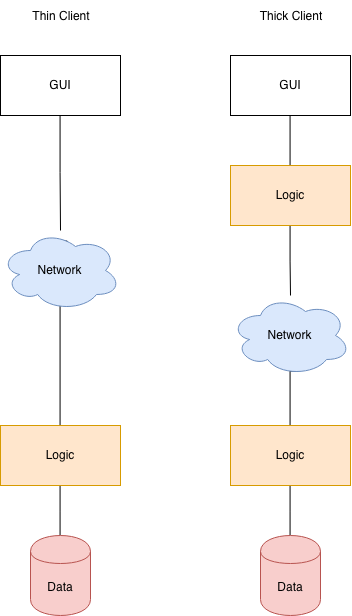
\includegraphics[width=0.4\textwidth]{./img/client_server.png}
    \hspace{0.05\linewidth}
    \centering
    \caption{Possible management of the client-server connection according to the MVC model. Thin or thick client.}
		\label{img:client_server}
    \end{center}
\end{figure}


\section{Other Design Decisions}
\subsection{User authentication}
In order to guarantee the confidentiality of user data, access to the system, both for standard users and for special users, takes place by entering a username and password.
The username used for access coincides with the email address used during registration.

\subsection{Password storing}
The passwords chosen by the users are saved in the database after being encrypted using a SHA512 algorithm.
In this way, the password to be used for accessing Data4Help services is not stored in plaintext in the user database, but it is a transformation from which, even with very powerful computers, it is very difficult to trace the original password.
In this way even using the normal Internet connection, if an intruder could pick up the string containing the password, he would not be able to trace the password used to access the service.

\subsection{Security in the transfer of information}
The transfer of data between the clients and the server is done using the most modern data encryption systems.
For example, the Web Server offers an HTTPS interface to the Web Browser.

\subsection{Maps}
In order to manage the rides offered by Track4Run, the external Google Maps service is used.
Longitude and latitude are used to locate a position within the map.
To ensure a better service to the user who is responsible for creating the race, it is also given the opportunity to create the route using the features provided by Google Maps such as search by address, search for places of public interest, and so on. In the database the race course will still be saved as a sequence of positions in terms of longitude and latitude.

\subsection{Emergency call}
Emergency calls are handled using an external service.
This ensures that even in the event that the data network is not available, or the application server is out of service, it is still possible to call for help.
In fact, the external service works via the Internet or, in the absence of a connection, via SMS.
When the Automated SOS application detects an anomaly, it invokes the external service and sends it the location of the device and a precompiled text containing information related to the health of the user.
This information is then sent to the rescue service by the external service.
